\documentclass[hyperref={pdfpagelabels=false},aspectratio=169]{beamer}


% Import packages
\usepackage{lmodern}
\usepackage{url}
\usepackage{tikz}
\usepackage{biblatex}
\bibliography{citations.bib}


% Load CambridgeUS theme and customize it to the SURF style
\usetheme{CambridgeUS}
\definecolor{SURF-gray}{HTML}{EFEFEF}         % Color taken from https://www.surf.nl/
\definecolor{SURF-orange}{HTML}{E67300}       % Color taken from https://www.surf.nl/
\setbeamercolor{palette primary}{use=structure, fg=SURF-orange, bg=SURF-gray}
\setbeamercolor{palette secondary}{use=structure, fg=SURF-orange, bg=SURF-gray}
\setbeamercolor{palette tertiary}{use=structure, fg=SURF-gray, bg=SURF-orange}
\setbeamercolor{structure}{fg=SURF-orange, bg=SURF-gray}
\setbeamercolor{title}{fg=SURF-orange}
\setbeamercolor{frametitle}{fg=SURF-orange}
\setbeamertemplate{title page}[default][]
\addtobeamertemplate{headline}{}{
\begin{tikzpicture}[remember picture, overlay]
    \node[anchor=north east, yshift=2pt] at (current page.north east) {
\includegraphics[height=1.6em]{images/SURF_logo.png}};
\end{tikzpicture}}


% Title page/footer info
\title{Container workload and orchestration in HPC}
% \subtitle{in high performance computing}
\author{Kees de Jong \& Maxim Masterov}
\institute[SURF]{}
\date{\today}


\begin{document}
    % Insert title slide
    \begin{frame}
        \titlepage
    \end{frame}

    % Customize title frame
    \AtBeginSection[]{
        \begin{frame}
            \begin{beamercolorbox}[center]{title}
                \usebeamerfont{title}\insertsectionhead\par
            \end{beamercolorbox}
        \end{frame}
    }

    % Insert table of contents slide, to ignore sections from the ToC and slides, use; \section*{Section no.1}
    \begin{frame}
        \frametitle{Table of contents}
        \tableofcontents
    \end{frame} 

    % Presentation slides start here
    \section{Introduction} 
    \begin{frame}
        \begin{itemize}
          \item In e.g. federated HPC infrastructures it is a challenge to maintain predictable software environments.
          \item With container technology there is also the question of orchestration (SLURM versus Kubernetes).
          \item The conclusion in this presentation in part based on related work \footfullcite{hpc-workloads-justin} \footfullcite{saha2018evaluation} \footfullcite{stackhpc-state-of-hpc}.
          \item Left out of scope in this presentation: Docker, udocker, Podman and Shifter.
        \end{itemize}
    \end{frame}
    \subsection{Research questions}
    \begin{frame}
      \begin{block}{Research questions}
      \begin{enumerate}
        \item How do container technologies compare in terms of usability, security, features, and performance on single and multi node compute jobs? 
        \item How to orchestrate/schedule compute jobs with containers? How do Kubernetes and SLURM compare with each other in terms of usability, scheduling features, and resource allocation?
      \end{enumerate}
      \end{block}
    \end{frame}
    \subsection{Container technologies}
%     \begin{frame}
%       \frametitle{Singularity}
%       \begin{itemize}
%         \item Most popular: 25,000+ systems are running Singularity at e.g. SURF, TACC, San Diego Supercomputer Center, and Oak Ridge National Laboratory.
%         \item Root privileges are not required to run and build containers.
%         \item Maps the UID/GID of the root user inside the container, to an unprivileged ID outside of the container.
%         \item However, with user namespaces enabled, the attack surface is widened \footfullcite{rhel-cve}.
%         \item Singularity uses SIF, which is a single-image format (smaller size than multi-layer images).
%         \item SIFs are treated like a binary executable, thus easily usable in SLURM job scripts.
%         \item Conversion tools available for OCI (Docker, Podman) to SIF (Singularity).
%       \end{itemize}
%     \end{frame}
%     \begin{frame}
%       \frametitle{Charliecloud}
%       \begin{itemize}
%         \item Charliecloud is minimal and lightweight and uses Linux user namespaces to run containers with no privileged operations or daemons.
%         \item It does not require root privileges to install the Charliecloud software or to run Charliecloud containers.
%       \end{itemize}
%     \end{frame}
%     \begin{frame}
%       \frametitle{Enroot}
%       \begin{itemize}
%         \item Enroot can be thought of as an enhanced unprivileged chroot.
%         \item Uses the same underlying technologies as containers but removes much of the isolation they inherently provide while preserving file system separation.
%         \item Notable features: scriptable configs and in-memory containers \footfullcite{nvidia-slurm-containers}.
%         \item Root privileges are required to build containers with enroot. Buildah may be used to build an OCI container and then convert to enroot format as an unprivileged user.
%       \end{itemize}
%     \end{frame}
%
%     \begin{frame}
%       \frametitle{SLURM}
%       \begin{itemize}
%         \item Provides a scheduling framework for starting, executing, accounting and monitoring (parallel) compute jobs with a defined, relative short runtime.
%         \item Provides the intelligence to manage queues and thus congestion of the compute resources.
%         \item Topology-aware, which is the intelligence to schedule jobs on nodes close together in the HPC cluster in order to keep latency low.
%         \item Agnostic towards container technologies and can handle most, if not all.
%       \end{itemize}
%     \end{frame}
%     \begin{frame}
%       \frametitle{Kubernetes}
%       \begin{itemize}
%         \item Primarily built for orchestrating containerized microservice applications.
%         \item Kubernetes may provide load-balancing and redundancy features to provide the maximum availability over a relative long runtime.
%         \item Microservices may be updated and maintained while in production \footfullcite{hpc-kubernetes-containers}.
%       \end{itemize}
%     \end{frame}
%     \subsection{Summary}
    \begin{frame}
%       \frametitle{Container technologies}
      \begin{block}{Singularity}
Secure and very popular container solution which allows to build and run containers without root.
      \end{block}
      \begin{block}{Charliecloud}
Secure container solution with a small attack surface due to its lightweight nature. Charliecloud also does not require root privileges to build and run a container.
      \end{block}
      \begin{block}{Enroot}
Mixes different isolation methods, while staying lightweight, with builtin GPU support. Cannot build containers without root (but can be done by Buildah).
      \end{block}
    \end{frame}
    \subsection{Container orchestrators}
    \begin{frame}
%       \frametitle{Container orchestrators}
      \begin{block}{SLURM}
Mainly focused on scheduling distributed parallel compute jobs with a defined end time. Where it is specialized in customizable efficient partitioning, queuing, accounting, monitoring and prioritizing jobs while being topology-aware
      \end{block}
      \begin{block}{Kubernetes}
Mainly focused on keeping microservices up and running without interruption. Kubernetes includes high-availability and load-balancing features between containers to mitigate congestion and latency for the microservice. There are developments towards support for HPC workflows.
      \end{block}
    \end{frame}
    
    \section{Method}
    \begin{frame}
%     \frametitle{Method}
    \begin{itemize}
      \item Goal: cover the majority of the possible use cases from fields like Computational Fluid Dynamics, Mechanical Engineering, Astrophysics, Machine Learning, and many others.
      \item We tested three linear solvers from PETSc library \footfullcite{PETSc2020overview}: CG, BiCGSStab and AMG.
%       \item The linear solvers were applied to a standard 3D Poisson problem with 7-point stencil and $500^3$ Degrees of Freedom (DoF).
      \item The chosen linear solvers cover the most frequently used algebraic operations from the back-ends of most scientific codes.
      \item Every test was executed on 1, 2 and 4 nodes with 24 MPI tasks per node with hyperthreading switched off (repeated 4x)
    \end{itemize}
    \end{frame}
%     \begin{frame}
% %     \frametitle{Method} 
%     \begin{table}[H]
%         \centering
%         \begin{tabular}{c c c}
%         \hline
%                 & Host machine & Container \\ \hline
%         OS      & RHEL7.8      & Ubuntu-18.04.4 LTS \\
%         GCC     & 7.3.0        & 7.5.0 \\
%         OpenMPI & 3.1.1        & 3.1.1 \\
%         PETSc   & 3.11.2       & 3.11.4 \\ \\
%         \end{tabular}
%     \end{table}
%     \end{frame}
    
    \section{Results}
    \subsection{Benchmarks}
    \begin{frame}
    \frametitle{Benchmarks CG}
    \begin{figure}[H]
      \centering
       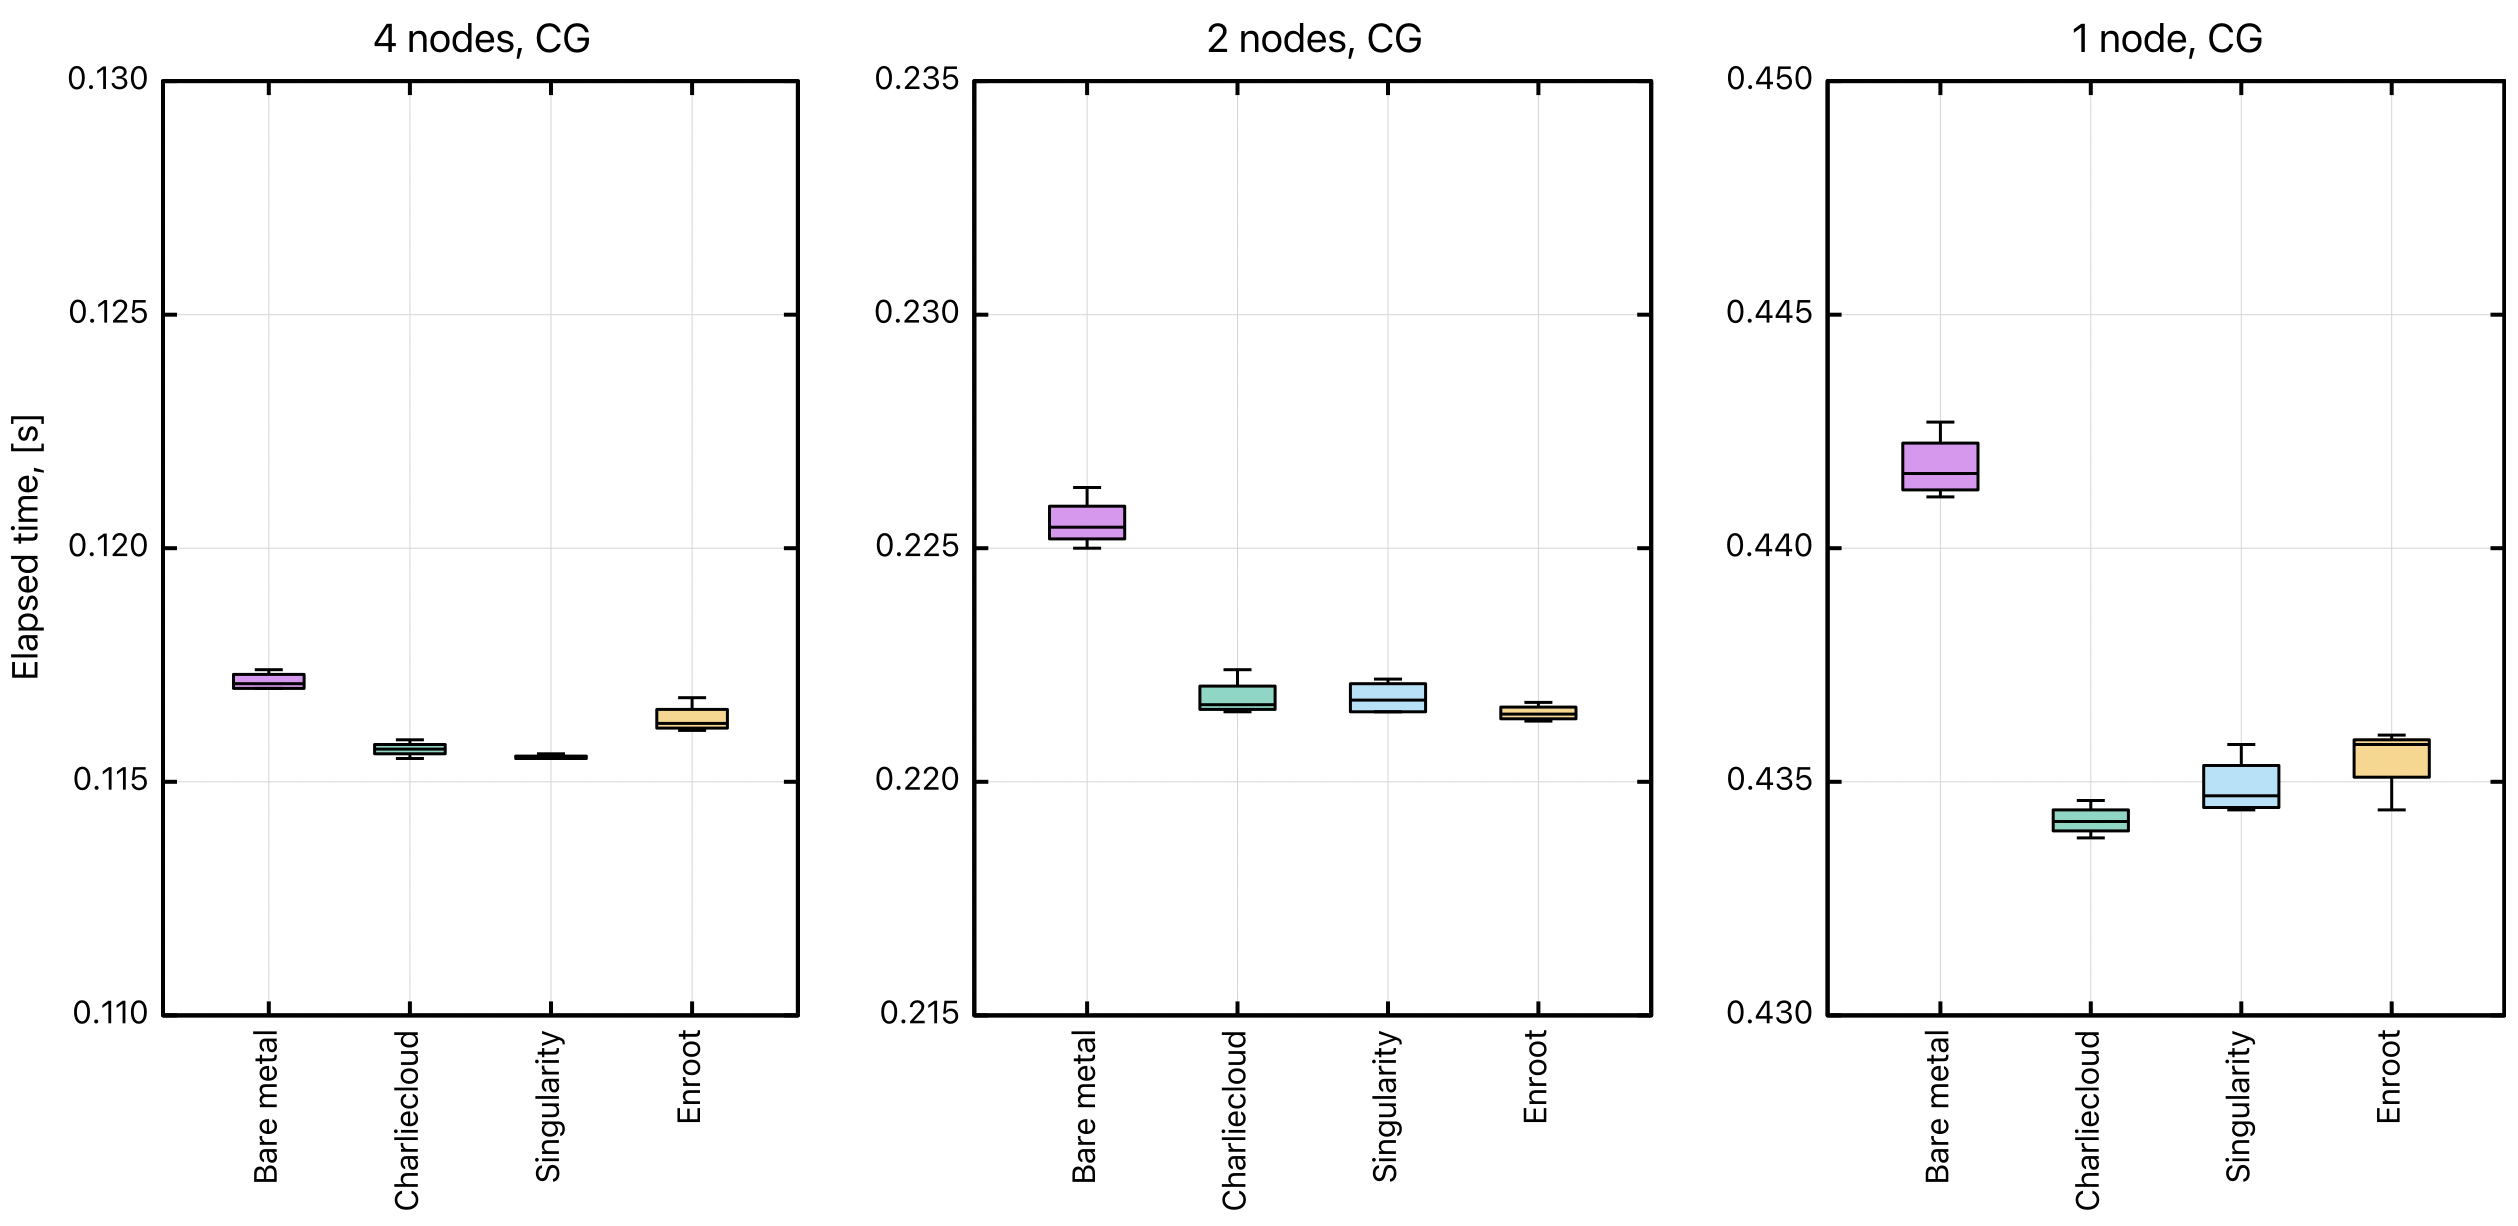
\includegraphics[width=0.9\textwidth]{images/cg.png}
      \label{fig:container_benchmarks}
    \end{figure}
    \end{frame}
    \subsection{Container benchmarks}
    \begin{frame}
    \frametitle{Benchmarks BiCGSStab}
    \begin{figure}[H]
      \centering
       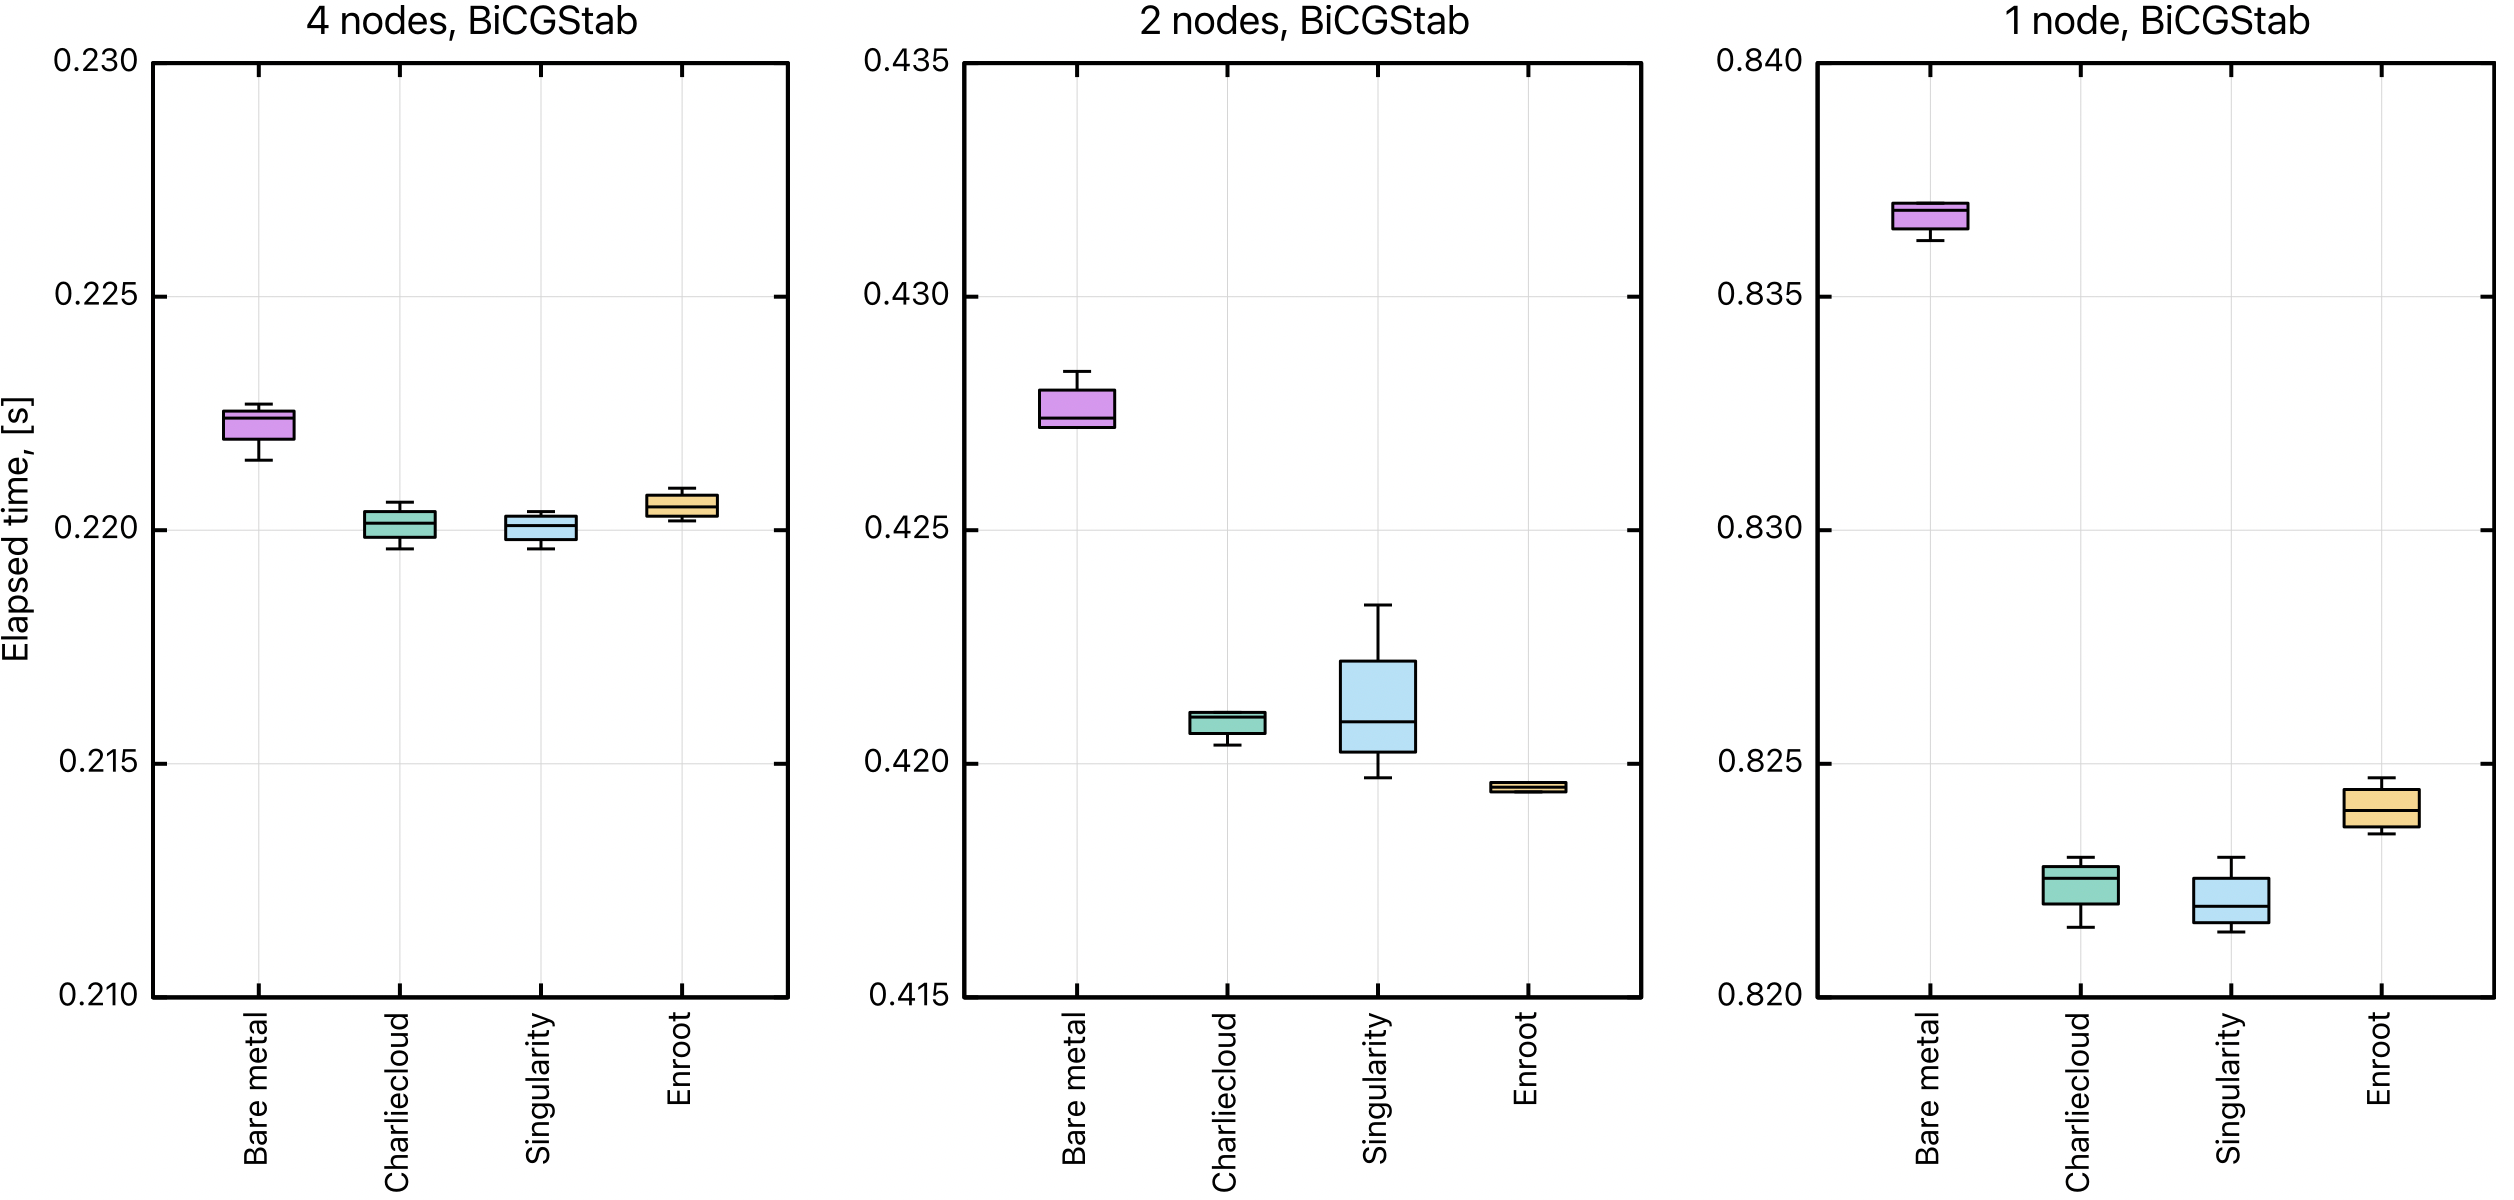
\includegraphics[width=0.9\textwidth]{images/bicgstab.png}
      \label{fig:container_benchmarks}
    \end{figure}
    \end{frame}
    \begin{frame}
    \frametitle{Benchmarks ML}
    \begin{figure}[H]
      \centering
       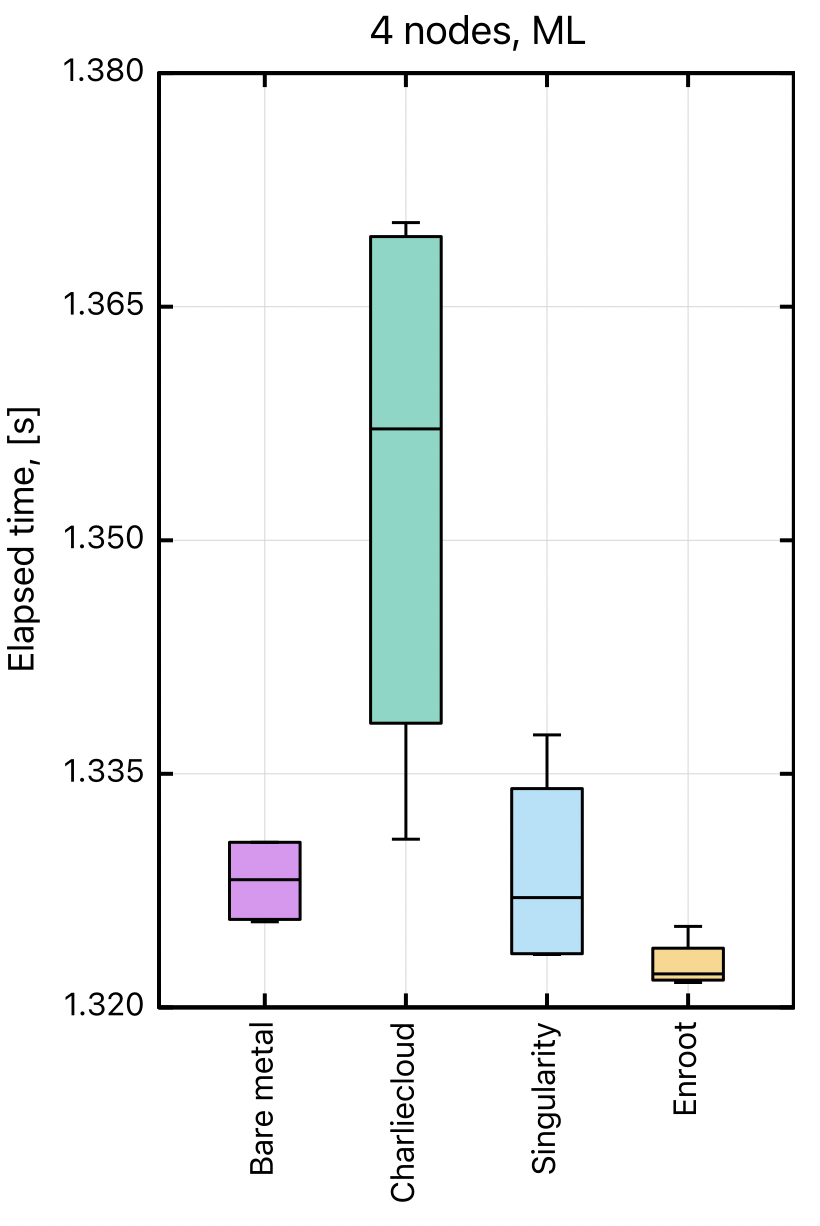
\includegraphics[width=0.3\textwidth]{images/ml.png}
      \label{fig:container_benchmarks}
    \end{figure}
    \end{frame}
    \subsection{Container technology in HPC}
    \begin{frame}
    \begin{block}{Introduction}
    Evaluation of the strengths and weaknesses of HPC-oriented container technologies. Based on an evaluation done by nVidia \footfullcite{nvidia-slurm-containers}. 
    \end{block}
    \end{frame}
    \begin{frame}
      \frametitle{Usability, features, and support for archived images}
      \begin{itemize}
        \item Singularity has 78 man pages. Charliecloud 20 manuals. Enroot had none.
        \item Online documentation was fine for all.
        \item Enroot had the least features, easier to start working with.
        \item Enroot lacked archived images (simplifies off-site utilization and execution of containers).
        \item Had to build and maintain our own RPMs for enroot\footnote{\url{https://fedorapeople.org/cgit/keesdejong/public_git/rpmbuild.git/tree/SPECS/enroot.spec}} \footnote{\url{https://fedorapeople.org/cgit/keesdejong/public_git/rpmbuild.git/tree/SPECS/pyxis.spec}}.
      \end{itemize}
    \end{frame}
    \begin{frame}
      \frametitle{SLURM and MPI support}
      \begin{itemize}
        \item Enroot provided a SLURM plugin (significantly simplifies HPC workflows).
        \item Enroot allows users to rely on system-defined rules for core affinity and core binding.
        \item All containers allowed to compile and execute MPI applications in the container.
      \end{itemize}
    \end{frame}
%     \begin{frame}
%       \frametitle{Support for recipes}
%       \begin{itemize}
%         \item Charliecloud allows the use of the industry-standard ``Dockerfile''.
%         \item Singularity uses a recipe files of its own format.
%         \item Enroot can only import images from container registries and add limited functionality with configuration files.
%       \end{itemize}
%     \end{frame}
%     \begin{frame}
%       \frametitle{Cross-platform}
%       \begin{itemize}
%         \item Singularity can be considered as a cross-platform container solution (some limitations on Mac).
%         \item Enroot and Charliecloud only work on Linux-based systems.
%       \end{itemize}
%     \end{frame}
    \begin{frame}
      \begin{figure}[H]
      \centering
      % \includegraphics[width=\textwidth/2]{images/kube_vs_slurm.png}
      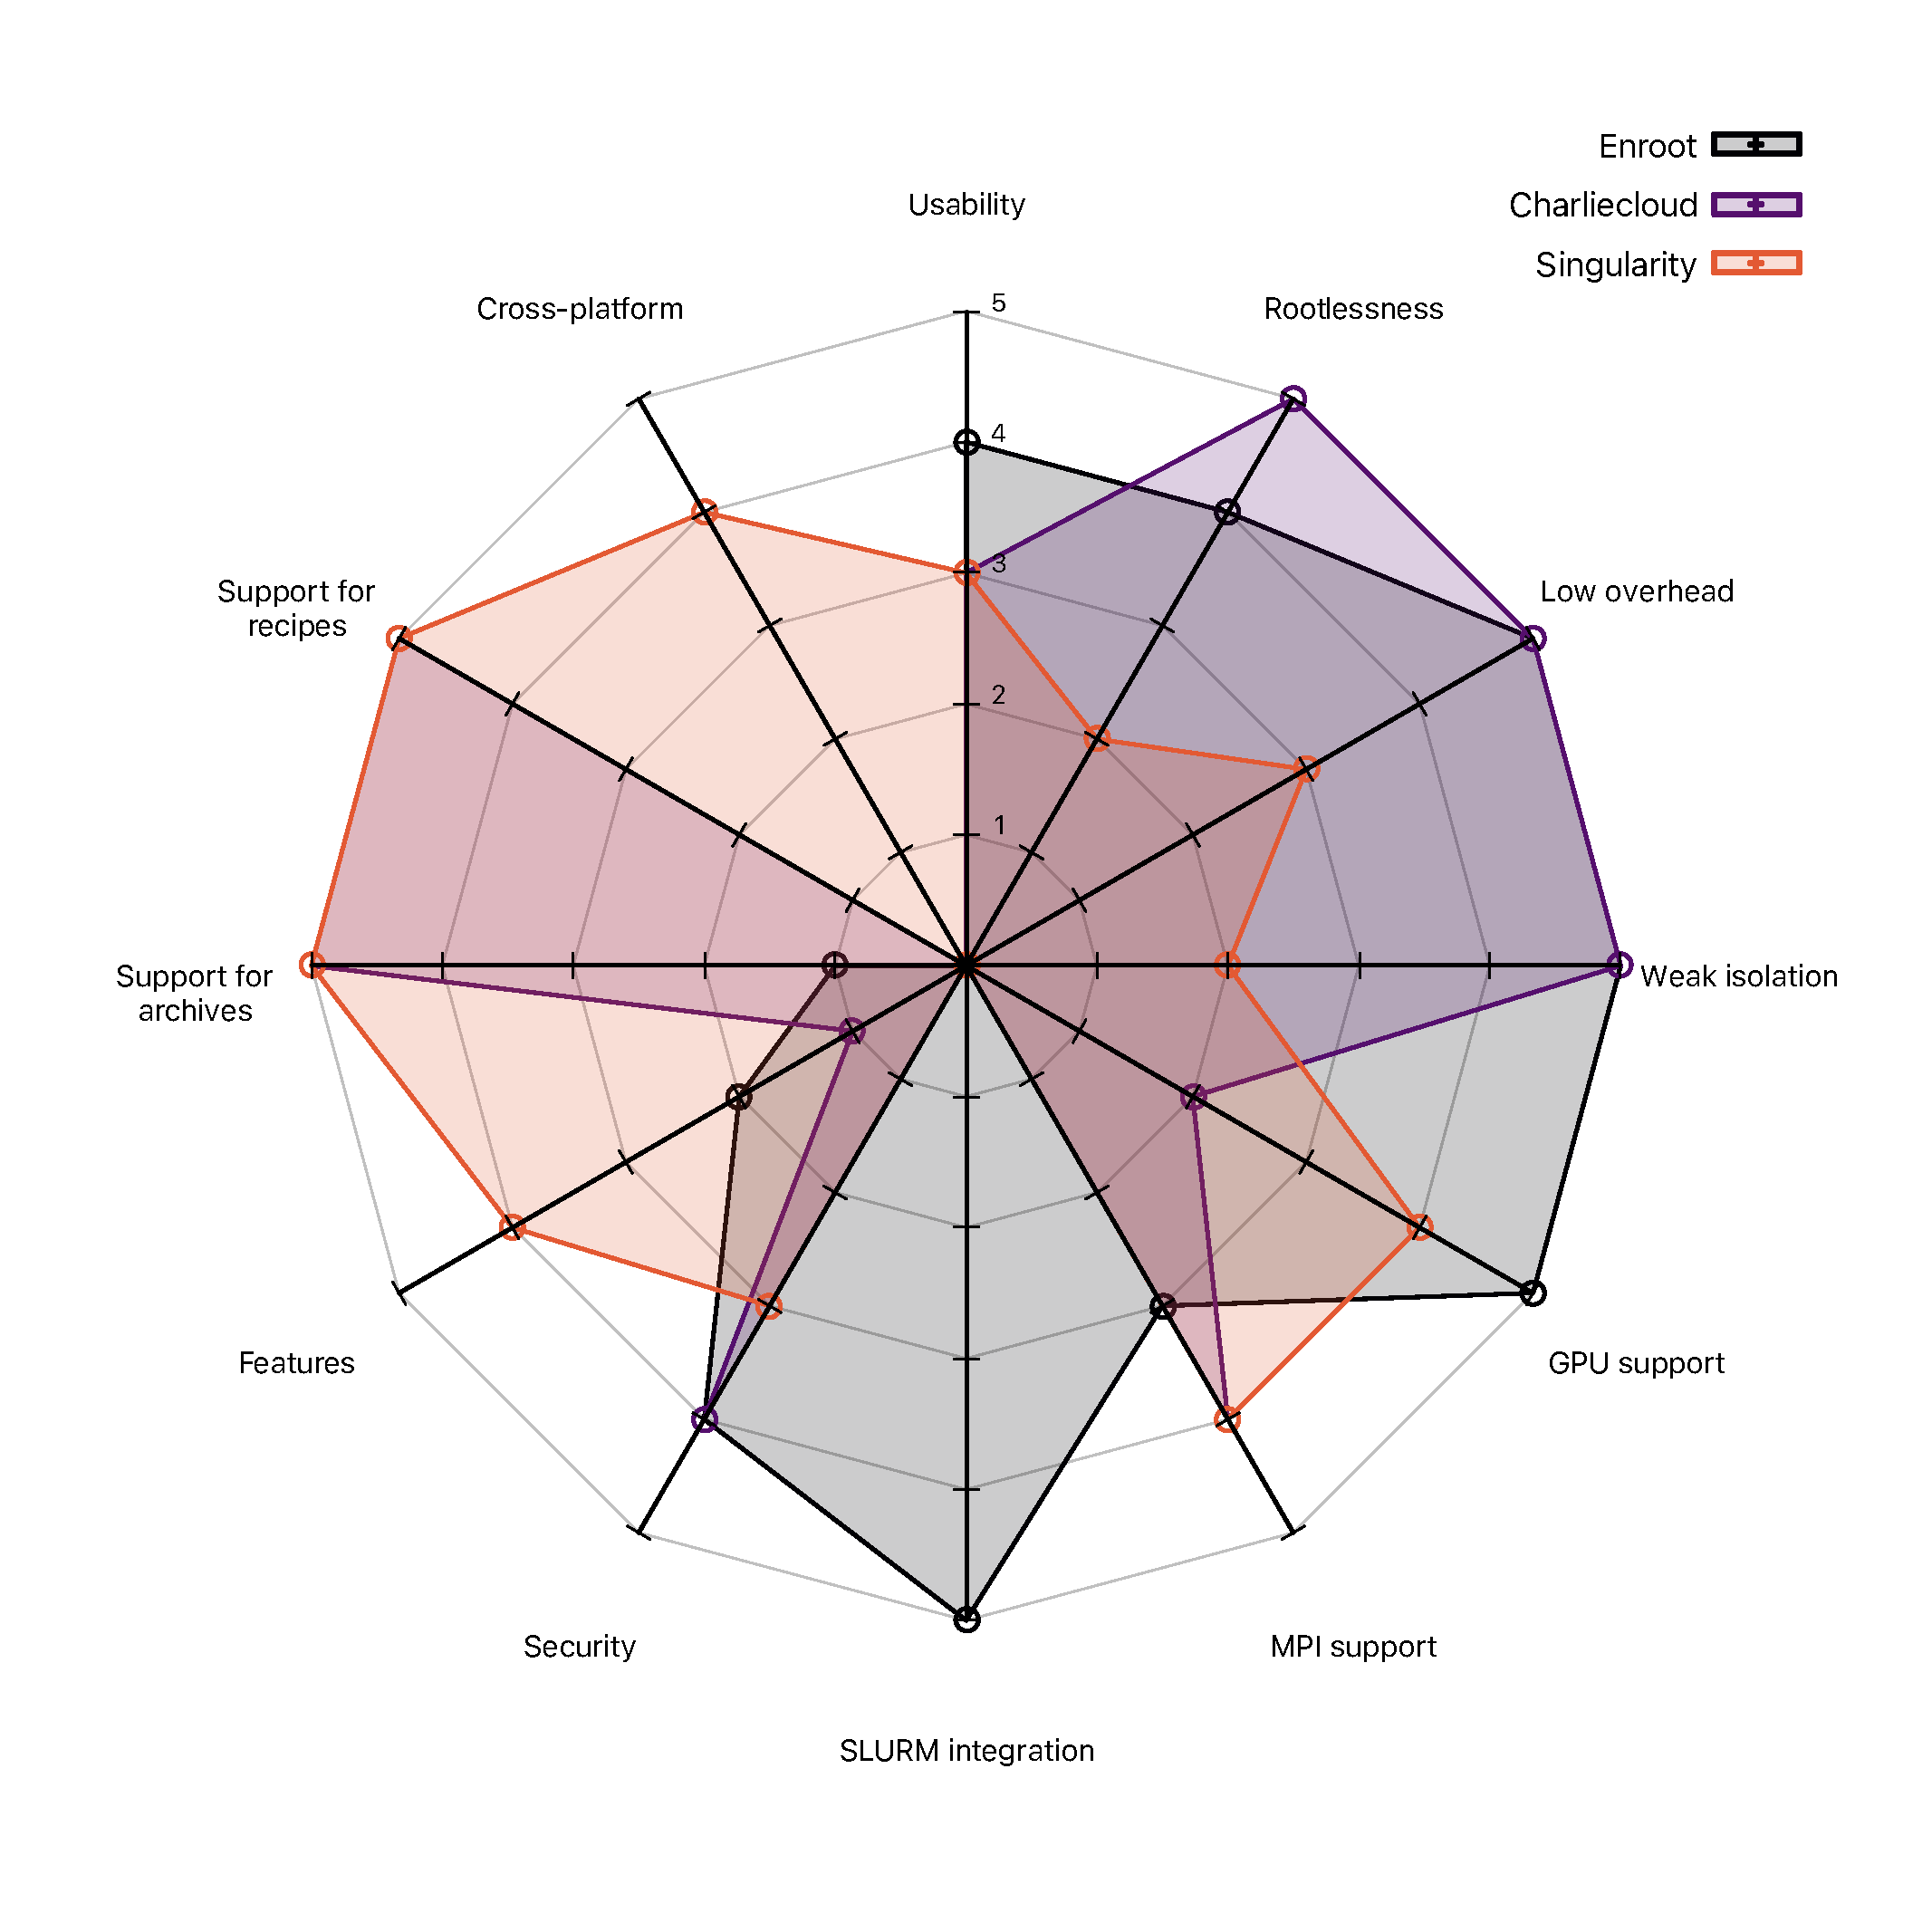
\includegraphics[width=0.55\textwidth]{images/containers_spider.pdf}
%       \caption{Strengths and weaknesses of SLURM and Kubernetes.}
    \end{figure}
    \end{frame}
    \subsection{Container orchestrators in HPC}
    \begin{frame}
      \frametitle{Kubernetes versus SLURM}
      \begin{itemize}
        \item Kubernetes is not performing optimally compared to SLURM.
        \item Typical HPC characteristics such as support for NUMA management, GPUs, InfiniBand, and FPGU is developing in Kubernetes.
        \item MPI support for Kubernetes, namely for large scale Machine Learning by the use of e.g. Kubeflow.
        \item Kubernetes lacks topology-aware scheduling.
      \end{itemize}
    \end{frame}
    \begin{frame}
      \frametitle{Deployment suggestions (1/2)}
      \begin{enumerate}
        \item Maintain separate infrastructures: setup different environment for Kubernetes workloads, comes with increased cost.
        \item Switch to hybrid workload managers: such as Univa Grid Engine Container Edition and IBM Spectrum LSF are adding native support for containers (Docker, Singularity and Shifter).
      \end{enumerate}
    \end{frame}
    \begin{frame}
      \frametitle{Deployment suggestions (2/2)}
      \begin{enumerate}
      \setcounter{enumi}{2}
        \item Use native job scheduling features in Kubernetes: known limitations in the context of HPC.
        \begin{itemize}
          \item Slower time-to-spool due to determining network plugins \footfullcite{futral2019method}.
          \item Worker pods have to be first provisioned before a controller pod could be provisioned via the batch job.
          \item Suffers latency from utilizing SSH for its communication protocol (SLURM uses MUNGE).
          \item Node availability determination slower (added layers of virtual network and custom dynamic DNS).
          \item And much more...
        \end{itemize}
      \end{enumerate}
    \end{frame}
    \begin{frame}
      \begin{figure}[H]
      \centering
      % \includegraphics[width=\textwidth/2]{images/kube_vs_slurm.png}
      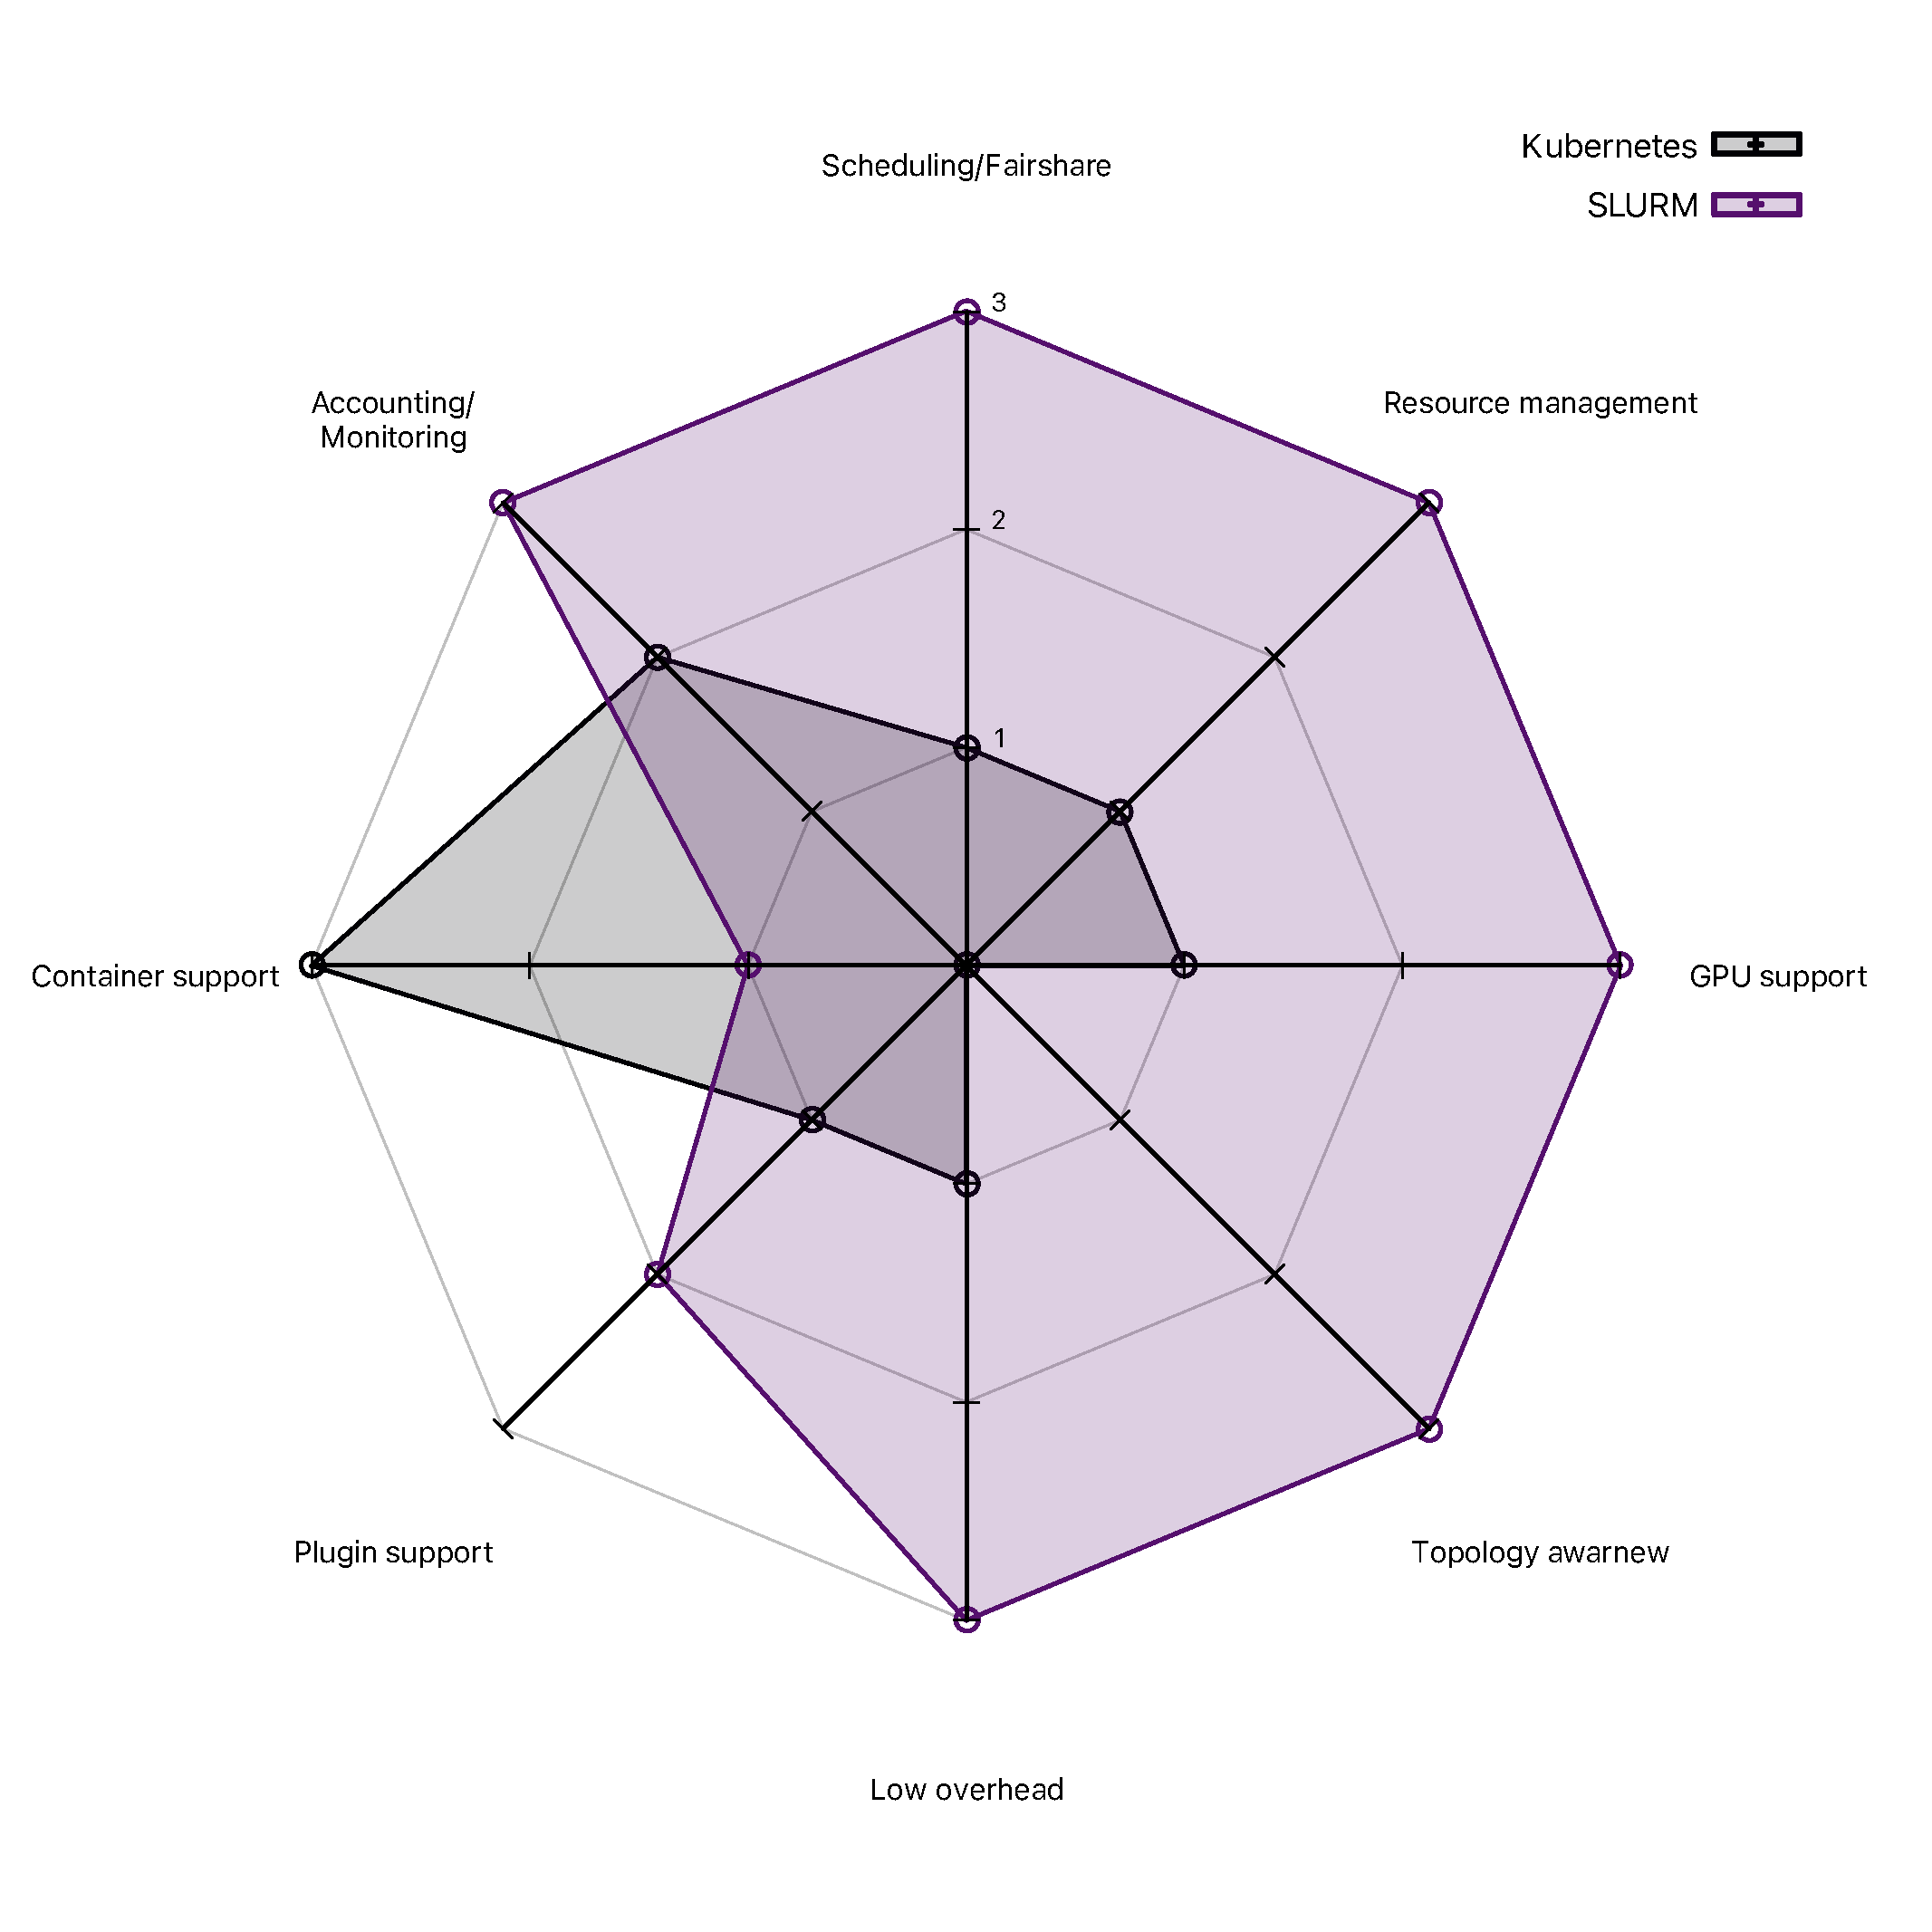
\includegraphics[width=0.55\textwidth]{images/kuber.pdf}
%       \caption{Strengths and weaknesses of SLURM and Kubernetes.}
      \label{fig:kube_vs_slurm}
    \end{figure}
    \end{frame}
    
    \section{Conclusion} 
    \begin{frame}
        \begin{itemize}
          \item Kubernetes excels at orchestrating containers, containerized HPC applications can be tricky to deploy on Kubernetes \footfullcite{kubenetes-blog-meets-hpc}.
          \item Significant developments under way for HPC features in Kubernetes.
          \item SLURM is designed to be used in HPC and excels for that reason.
          \item Singularity and Enroot score best overall. Enroot excels with (nVidia) GPU workloads. Charliecloud looks very promising as well.
          \item Traditional HPC and Kubernetes co-existence is possible. However, there should be a valid use case for such a more complex and expensive setup \footfullcite{cloudy-hutch}
        \end{itemize}
    \end{frame}
    \begin{frame}
    Full report can be downloaded by scanning the QR code or visit the short URL\footnote{\url{https://bit.ly/3pTNfIZ}}
      \begin{figure}[H]
      \centering
      % \includegraphics[width=\textwidth/2]{images/kube_vs_slurm.png}
      
\includegraphics[width=0.3\textwidth]{images/frame.png}
%       \caption{Strengths and weaknesses of SLURM and Kubernetes.}
      \label{fig:kube_vs_slurm}
    \end{figure}
    \end{frame}
\end{document}
